\documentclass[12pt,a4paper,twocolumn]{article}
\usepackage{hw}
\usepackage{subcaption}
\usepackage{multicol}

\graphicspath{ {.} }

\title{\vspace{-1cm}\Large\textbf{{Which Sensor to Use - Single or Composite Sensor?}}}
\author{Zong Fan}
\date{Bioengineering, UIUC}

\begin{document}
\maketitle
% \multicols{2}

\section{Introduction}
A company meets a problem. There are 2 kinds of candidate linear time invariant (LTI) sensors they'd like to use in their product. The first sensor consists of a single component and the second one has 4 composite sensors with different resonant frequencies but sharing the same damping factor $\zeta$. The detailed engineering parameters are shown in Figure ~\ref{fig:1}. The sensor would be applied to measure a sequence of square wave oscillations with increasing frequency. Since sensor 2 costs twice that of sensor 1, we need to conduct analytics to make a good tradeoff evaluation between model performance and cost. 

\begin{figure}[!ht]
    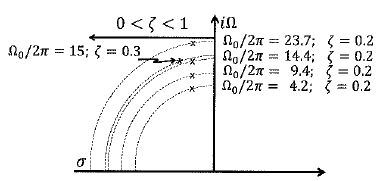
\includegraphics[width=\columnwidth]{lab2_pole.png}
    \caption{Pole-zero plot describing the 2 LTI sensors\cite{insana2020biomedical}. Resonant frequencies $\Omega_0/2\pi$ and damping factors $\zeta$ are indicated for sensor 1 ($\ast$) on the left and for sensor 2 ($\times$) on the right.}
    \label{fig:1}
\end{figure}

\section{Methods}
\subsection{Data}
The data we used to evaluate the performance of sensors is manually synthesized which is a sequence of square wave objects. As shown in Figure ~\ref{fig:2}, its duration is 10s and its magnitude is 1. Its oscillation frequency increases along time, that is 1 $s^{-1}$ in the first 4s, 2 $s^{-1}$ from 4s to 6s, 4$s^{-1}$ from 6s to 8s, 8$s^{-1}$ from 8s to 10s. 

\begin{figure}[!ht]
    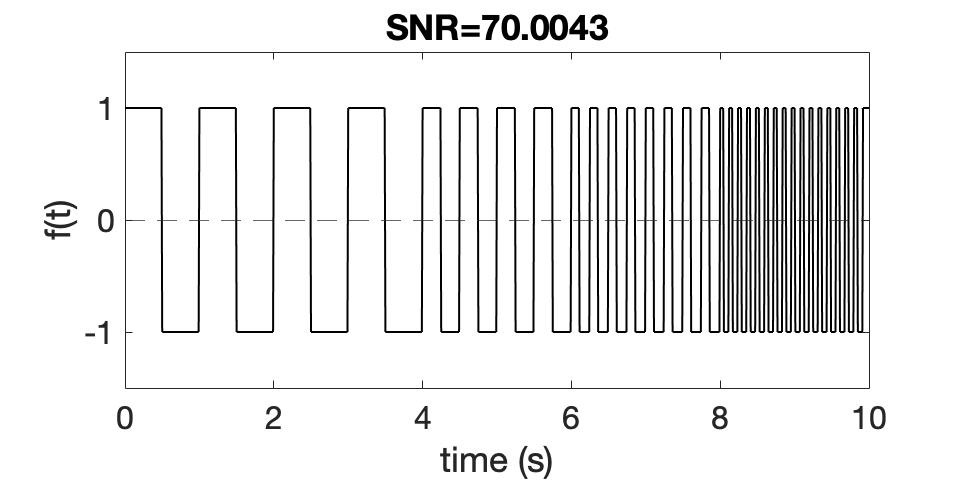
\includegraphics[width=\columnwidth]{lab2_sig.png}
    \caption{Input square wave signal for sensors to model.}
    \label{fig:2}
\end{figure}

\subsection{Analytics Pipeline}{\label{ap}}
According to acoustic sensors section in \S 11.2\cite{insana2020biomedical}, we're able to evaluate the powerfulness of a sensor by comparing the frequency distribution derived from its impulse response. Both peak magnitude and bandwidth of the frequency spectrum show important characteristics of sensors, corresponding to sensitivity and temporal resolution respectively. Since the spectrums of the 2 sensors are normalized which means they have the same peak spectral value, The major information for comparison would be the bandwidth of the frequency spectrum. To get bandwidth information, we would conduct analytics in the following steps: 
\begin{itemize}
    \item Compute impulse response of single sensor $h_1(t)$ and composite sensor $h_4(t)$ by equation 11.14\cite{insana2020biomedical}. \\
    $h(t)=\cfrac{k_0e^{-\Omega_0\zeta t}}{\Omega_0\sqrt{1-\zeta^2}}sin(\Omega_0\sqrt{1-\zeta^2}t)step(t)$
    \item Use Fourier transform of impulse response $h(t)$ to get spectral density function: $G(u)=\mathcal{F}\{g(t)\}$. We could measure bandwidth here. 
    \item Use convolution equation to restore input signal via $g(t)=[h*f](t)$. Then use mean squared error (MSE) to measure the effect of $h(t)$. 
\end{itemize}

\begin{figure*}[!ht]
    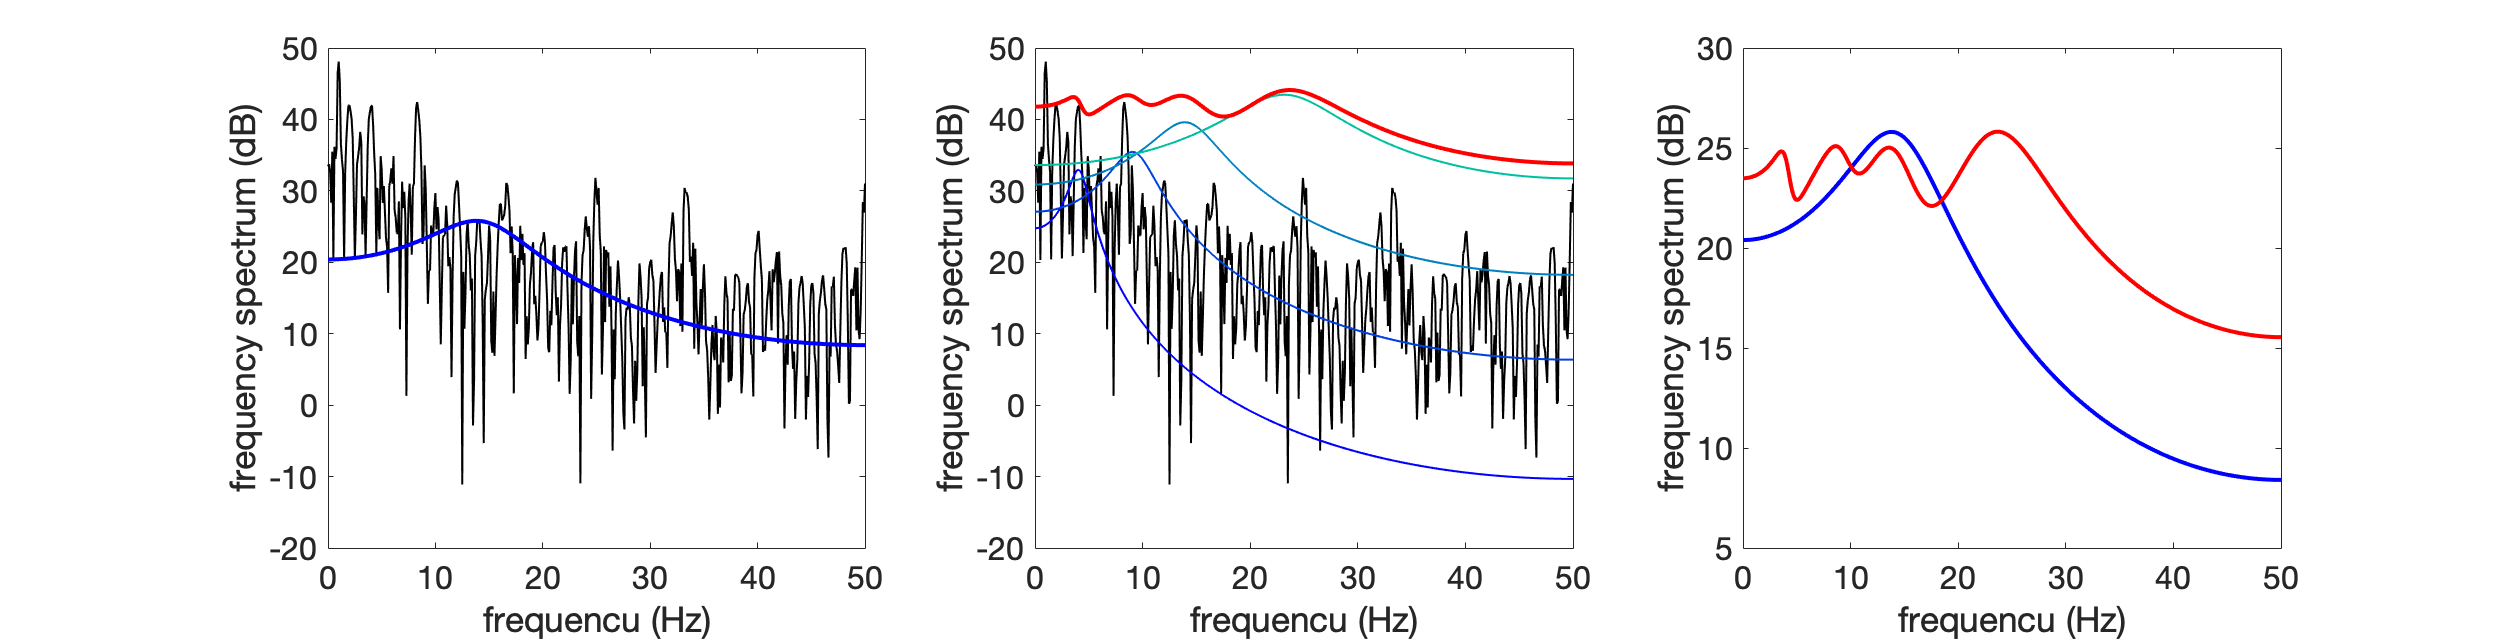
\includegraphics[width=\textwidth]{lab2_spectrum.png}
    \caption{Frequency spectrums of senor 1 and 2. In the left plot, the black curve is for input signal $\mathcal{F}\{f(t)\}$ while the blue curve is for normalized impulse response of sensor 1. In the middle plot, the black curve is for input signal while the blue curves with increasing hues are for normalized impulse response of each sub-sensors of sensor 2. The red curve is the weighted sum of frequency spectrum. In the right plot, the blue and red curves represent frequency spectrums that are normalized to have the same peak spectral value.}
    \label{fig:4}
\end{figure*}

\subsection{Metrics}
To evaluate how well the input signal is restored, MSE is computed to measure the distance between real input signal $f(t)$ and measured output $g(t)$.\\
$MSE=\bint{0}{t}dt (f(t) - g(t))^2$

\section{Results}
\subsection{Impulse responses and frequency specturms}
We compute the impulse response based on the first step described in section \ref{ap}. For sensors, we need to compute the individual impulse response of each sub-sensor first and then combine them into normalized weighted sum with given weights $\mathbf{w}^T=(1,2,4,8)$.
As shown in Figure ~\ref{fig:3}, the impulse response of sensor 2 has higher response magnitude and shorter period of oscillation compared with sensor 1, indicating it may have better effect on repressing ringing phenomenon.
\begin{figure}[!ht]
    \centering
    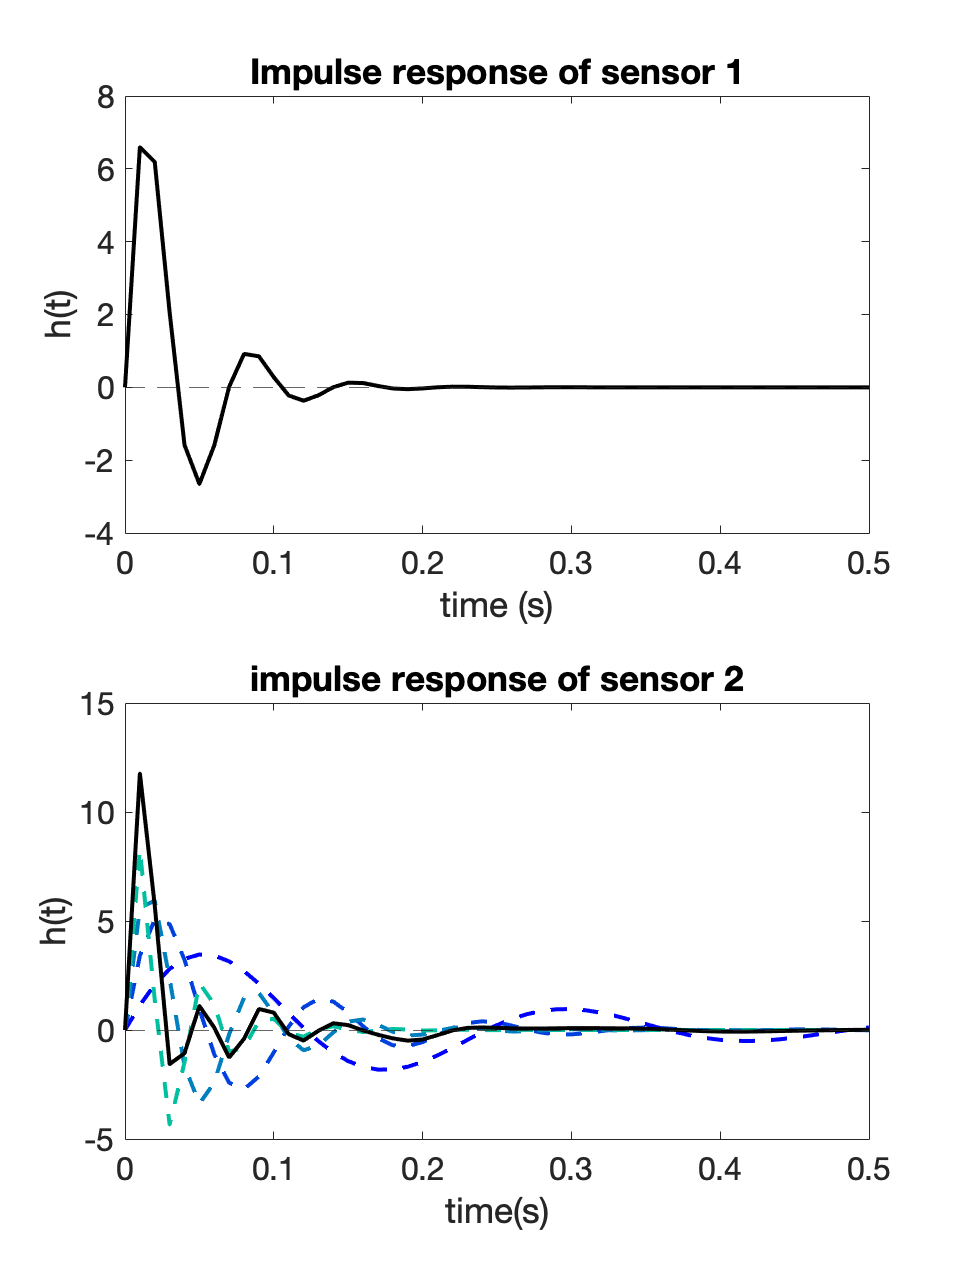
\includegraphics[width=0.9\columnwidth]{lab2_impulse.png}
    \caption{Impulse function of sensor 1 and sensor 2. The top plot indicates the impulse response of sensor 1; In the bottom plot, the blue dashed curves with increasing hues correspond to sub-sensors with increasing resonant frequencies from $h_a(t)$ to $h_d(t)$ while the black curve is the normalized weighted sum of impulse responses from sub-sensors.}
    \label{fig:3}
\end{figure}

Then we compute the frequency spectrum of each sensor as the second step in section \ref{ap} by applying Fourier transform to both input signal $f(t)$ and impulse response $h(t)$. As shown in Figure ~\ref{fig:4}, we could see that sensor 2 has significant wider bandwidth in the frequency spectrum ($H_4(u)$) of impulse response. Sensor 1 only has one peak at 15Hz, while sensor 2 has 4 peaks at 4.2, 9.4, 14.4, 23.7Hz. Such wide bandwidth makes sensor 2 to respond more quickly to the transitions of input signal no matter in low-frequency part or in high-frequency part. Besides, we also find that the $H_d(u)$ hits the highest peak value which means this sub-sensor has more energy to give higher sensitivity for high-frequency signals.

\subsection{Evaluate the restoration of input signal}
The most direct way to evaluate the performance of thesensor is to measure how well it could restore to input signal with that particular impulse response function $h(t)$. According to the third step in section \ref{ap}, we measure the MSE distance between the input signal $f(t)$ and the restored signal $[h*f](t)$ via convolution. Since the input signal has 4 kinds of frequencies, we decompose it and compare each of them individually. 

As shown in Figure \ref{fig:5}, we observe that sensor 2 has less ringing on the transition edges. In addition, when the input signal has higher frequencies, the restored signal by sensor 1 is more round-shaped rather than square-shaped compared with sensor 2. This phenomenon is consistent with the truth that the MSE distances from the high-frequency part are significantly larger than those from the low-frequency part. For the lowest frequency signal, the two sensors almost have identical performances. For signal across all frequencies, the overall MSE from sensor 1 is 0.3 and is 0.279 from sensor 2, which means sensor 2 has 7\% improvement in keeping signal fidelity. If we only focus on the highest-frequency part, the MSE would reduce from 0.671 to 0.607, achieving 10\% improvement.

\begin{figure}[!ht]
    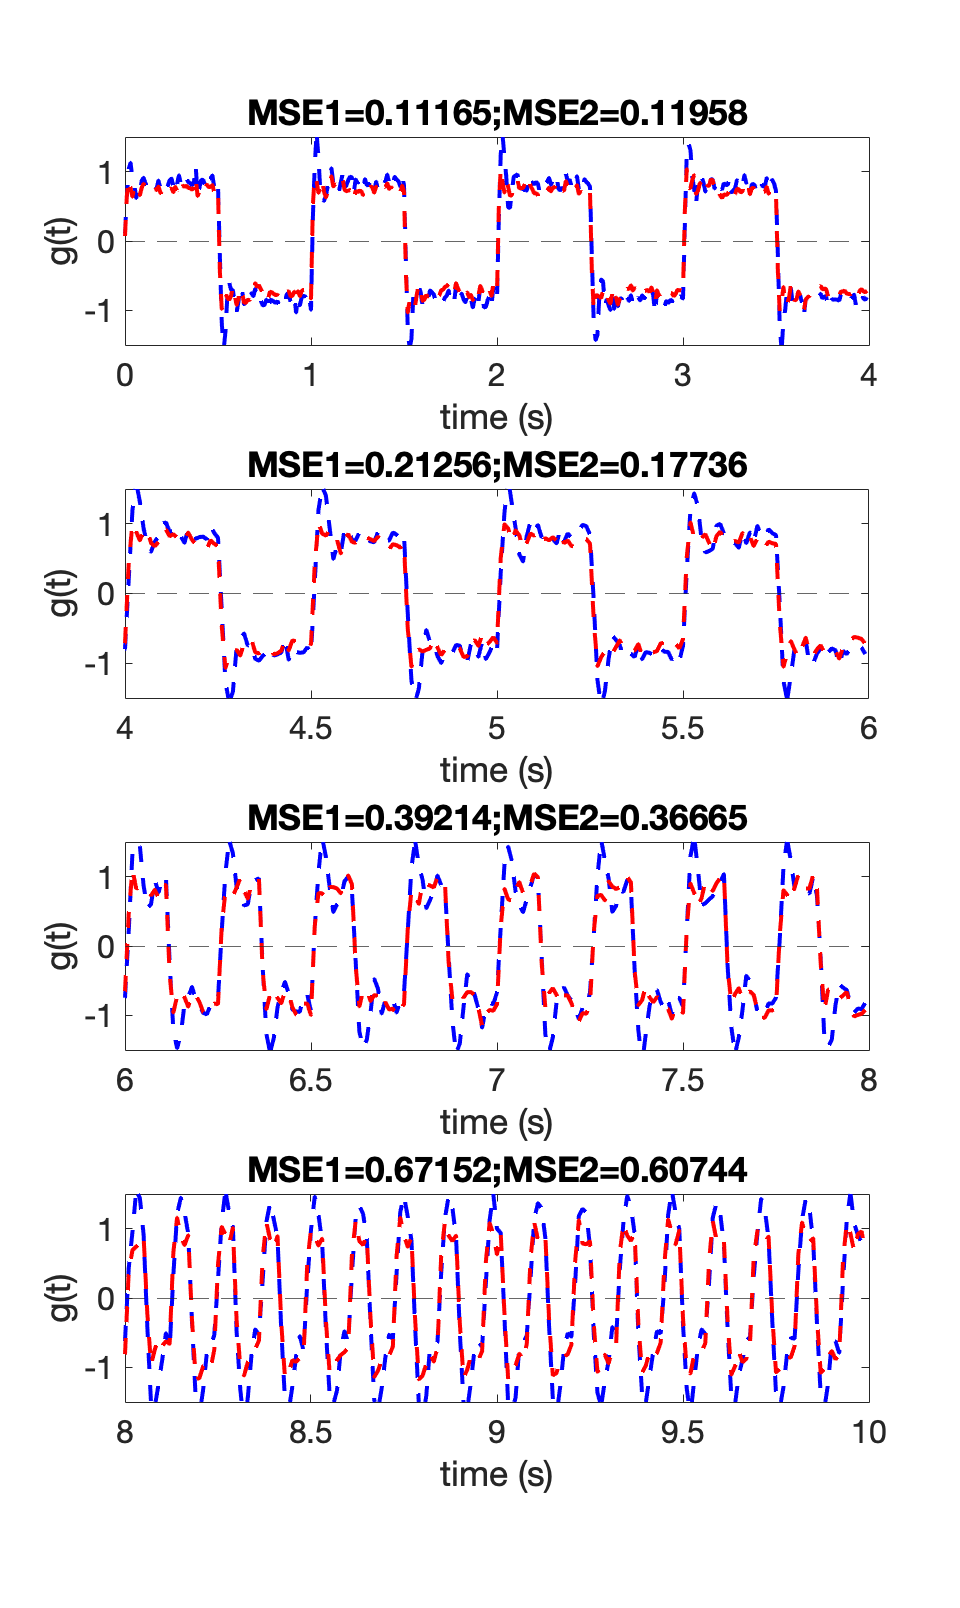
\includegraphics[width=\columnwidth]{lab2_mse.png}
    \caption{Comparison of restore signal between sensor 1 and sensor 2. The blue curves are restored signal from sensor 1 and the red curves are from sensor 2. The plots from the top to the bottom correspond to the input signal from 0s to 4s, 4s to 6s, 6s to 8s, and 8s to 10s with oscillation frequency from 1 to 8.}
    \label{fig:5}
\end{figure}

\section{Conclusion \& Discussion}
Till here, we have a clear landscape about the characteristics of the single sensor and composite sensor, including 1) sensor 2 has wider bandwidth to respond quickly to the transitions of signals; 2) sensor 2 has higher sensitivity on high-frequency signal, which achieves as much as 10\% improvement in the fidelity of restoring input signal; 3) the performances of sensor 1 and sensor 2 are almost identical in low-frequency signal. 

However, is this information enough to guide us to choose the suitable sensor for usage? Not necessarily. We still need a detailed task to balance the tradeoff between cost and performance. For example, if our task is to detect whether the machine is receiving low-frequency signal above a certain threshold so that some particular following functions would be activated, sensor 1, the cheaper one, would absolutely meet our demand. However, if we need to measure high-frequency signal accurately and repress annoying noise as much as possible for following operations, or the machine needs to process signals having a wide frequency spectrum, sensor 2 is superior in these cases. 

\bibliographystyle{abbrv}
\bibliography{final_lab}
% \end{multicols}
\end{document}